\chapter{Introducing Norms to Agents: Normative Advisors}
\label{ch:normative_advisors}
\textcolor{red}{ABSTRACT REWRITE and SOME TONE CHANGE IN THE BODY} This chapter introduces a modular architecture for integrating norms in autonomous agents and multi-agent systems. As the the interactions between norms and agents can be complex, this architecture utilizes multiple programmable components to model concepts such as adoption of multiple personal and/or collective possibly conflicting norms, interpretation and qualification between social and normative contexts, possibility of intentionally (non-)compliant behaviors and resolving conflicts between norms and desires (or other norms). The architecture revolves around \emph{normative advisors} that act as the bridge between intentional agents and the institutional reality. As a technical contribution, a running implementation of the architecture is presented based on the ASC2 (AgentScript) BDI framework and eFLINT norm reasoner. 


\section{Introduction}
Designing software agents that can reason with norms---technical instances of \emph{normative agents}---requires evidently having a suitable computational model for reasoning with norms. This is a challenging task because norms are more than a set of formal rules extracted from a legislative text: they emerge from multiple sources with different degrees of priority, they require interpretation to be encoded and qualification to be applied within a social context. Furthermore, they continuously adapt, in both expression and application~\cite{Boella2014APractice}. 

Previous proposals to embed norms in multi-agent-systems (MAS) have focused on extending the agent architecture (usually based on beliefs-desires-intentions, or BDI) to allow for forms of normative reasoning \cite{Dignum2002MotivationalNorms,Broersen01theboid,Tufis2017,Criado2010TowardsCompliance}. Two general approaches can be identified in the literature. One can encode norms as facts, and axiomatize normative reasoning with dedicated rules, to leverage the inferential engine provided with the agents; in this case, no modification needs to be applied to normative agents compared to non-normative agents. In contrast, in frameworks like BOID~\cite{Broersen01theboid} or B-DOING~\cite{Dignum2002MotivationalNorms}, explicit normative components like obligation (O) are considered to play a role in the decision-making cycle, requiring a modification of said cycle. In both cases, the agent is considered as a unity from an execution point of view: the agent script is a program, usually interpreted, and its internal reasoning cycle executed by a single thread. This work starts from the observation that this constraint is a rather strong one, not needed, and not always the most suited. Rather than an event-based reactive architecture based on a single event-queue and scheduling, individual agents may be each implemented as a system of concurrent actors, provided with some form of organization (e.g. event dispatching) and interaction mechanism (e.g. messaging).% Clearly, the overhead of complexity required for setting up a correct coordination amongst computational units, and for enabling and/or performing debugging, does not provide a good case for such construction. 

Normative agents offer a context in which this way of design gains more viability, for several reasons. On \textit{content} level, multiple normative sources may be concurrently relevant, and/or multiple interpretations of the same normative sources may be available (e.g. retrieved from previous cases), and these may be possibly conflicting. Enabling to maintain those in a modular fashion is a suitable precondition for update/adaptation actions, where norms can be changed on the fly, and agents may decide at run-time e.g. to change the relative priority between normative components. On \textit{method} level, there is still an ongoing debate on what is the most adequate representation model for norms, and on proper methods for normative reasoning (e.g. managing conflicts). Enabling the recourse to external tools, and supporting programmability of the coordination level, greatly empowers modelers/programmers/designers to test and compare different choices. Finally, at \textit{functional} level, most of the knowledge instilled in norms concerns a full social system; only a part is contingently relevant to the agent. Designing the system so that it distributes the inferential load at best (and at need) externally from the decision-making is seemingly the most efficient option.

\paragraph{Contribution}
For these reasons, this work proposes an abstract architecture that encapsulate norms (namely encoded in terms of normative relationships of Hohfeld's framework) in a MAS. The architecture centers around \textit{normative advisors} that can be utilized by (other) agents in the MAS as a sort of council about the institutional state of affairs and normative relations between agents, highlighting the mapping between the social and institutional views of the environment. Agents may resort to personal or to collective advisors, depending on the decentralization constraints set up by the designer.   
%
As a technical contribution, we present a practical implementation of this architecture that relies on the AgentScript BDI framework (ASC2) \cite{MohajeriParizi2020} for programming agents, and norm specification framework eFLINT \cite{VanBinsbergen2020EFLINT:Specifications} for encoding norms. 
%



\paragraph{Related works}
% There are multiple existing works in the literature on this topic. 
The B-DOING framework \cite{Dignum2002MotivationalNorms} explores logical relations between belief, desire, obligation, intention, norms and goals in agents and their interactions like conflicts and possible appraoches to balance them in agent's behavior. Similarly, the BOID architecture \cite{Broersen01theboid,Pandzic2022BOID} proposes a belief, obligation, intention and desire architecture with a feedback loop to take the effects of actions before committing to them. These studies (and many others, e.g., \cite{Deljoo2018APlaces,Tufis2017}) propose extensions to the BDI architecture to add (regulative) norms as part of the agents' mind and to resolve conflicts with pre-defined rules as part of the agent's reasoning cycle.


The normative BDI architecture presented in \cite{Criado2010TowardsCompliance} proposes different contexts for an agent: mental, functional and normative contexts, plus ``bridge rules'' between them. Their approach aims at creating maximally compliant agents and focus on solving conflicts between norms at the time of adoption by using pre-defined conflict resolution rules. The work presented in \cite{Cardoso2021ImplementingBDI} propose an approach for ethical reasoning in MAS by programming \textit{ethical governors}. Their method is close to ours in the sense that they also take advantage of extra agents in a MAS, but they focus on machine ethics used in the decision-making of one agent.


\paragraph{Structure of the document}
Section~\ref{sec:background} gives background on the core components that the proposal uses, providing some detail on the AgentScript/ASC2 and eFLINT frameworks. Section~\ref{sec:framework} lays out the theoretical framework for the proposed architecture, whereas Section~\ref{sec:implementation} describes details of its implementation. Section~\ref{sec:discussion} reflects on the capabilities of our implementation, suggests future directions, and draws connections with related work.


\section{Core components\label{sec:background}}

\begin{figure}[!tb]
    \centering
    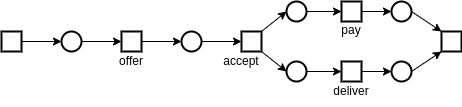
\includegraphics[width=0.5\textwidth]{ch_eumas/sale-drawio.png}
    \caption{Sale transaction as a \textit{Petri net} workflow}
    \label{fig:sale}
\end{figure}
%

To illustrate our approach, we will consider as a running example a marketplace environment consisting of buyer and seller agents. This target domain can be seen as an abstract model of many real-world domains, e.g. data market-places and more in general data-sharing infrastructures, electronic trading infrastructures, etc. The process model of a individual sale transaction---prototypical example of bilateral contract---can be represented as a workflow through a Petri-net, presented in Figure~\ref{fig:sale}. A seller offers a buyer an item for a certain price. If the buyer accepts the offer, then the seller is expected to deliver the aforementioned item to the buyer, and the buyer is expected to pay the seller the agreed upon price (in any order). The workflow is a simplified representation of the normative mechanisms in place during an actual sale transaction. Furthermore, it does not consider the intentional aspects on the agents during the transaction, e.g. based on which desires or goals the agents may be willing to engage in the transaction, as these concepts stay external to norms.
%It does not consider \textit{why} the agents may be willing to engage with the transaction (purpose, on which bases, expectations, etc.), nor the various normative relationships dynamically created along the process in order to guide the coordination between the parties. 
%To capture those, we need to further increase the design granularity of our target system.
%
\subsection{Intentional agents}
The intentional agents defined in this chapter intuitively are implemented in ASC2. 
%\gio{[There are a few things which are not explained of the code. e.g. a couple of words on the initalization of the normative advisor, and more importantly on \texttt{\#achieve}... what does it serve for? Has it any connection with the speech act? I would take one plan rule (e.g. \texttt{+offer}) and explain it in detail. Overall the granularity/size of this paragraph should be similar to the one of eFLINT.]}
Continuing with the example, Listing~\ref{asc:buyer}, presents the script of a buyer agent. The initial beliefs (lines 1-3), initial goals (line 5), and plan rules (line 7 and onwards) are the components of the script. The script is further explained in Section~\ref{sec:scenario}. 

% Intentional agents are generally approached in the computational realm via the \textit{belief-desire-intention} (BDI) model \cite{Rao1995}, % is used as the reference to define intentional agents. 
% %Having its roots in a theory of mind \cite{bratman1987intention}, the BDI model has been 
% %investigated in the literature as basis 
% to specify computational agents acting in dynamic environments with rational behavior.
% % uses taxonomies that are used typically to address human behaviour to describe agents.
% The BDI model refers to three human mental attitudes % used to describe human behavior 
% \cite{bratman1987intention}: \textit{beliefs} are the factual and inferential knowledge of the agent about itself and its environment; \textit{intentions} are the courses of action the agent has committed to; \textit{desires}, in their simplest form, are objectives the agent wants to accomplish. In practice, BDI agents also include concepts of \textit{goals} and \textit{plans}. Goals are concrete desires, plans are abstract specifications for achieving a goal, and intentions then become commitments towards plans. Multiple programming languages and frameworks have been introduced to operationalize the BDI model, such as AgentSpeak(L)/Jason~\cite{RaoAS1996,Bordini2005}, 3APL/2APL~\cite{Dastani2007}, Astra~\cite{Dhaon2014} and AgentScript/ASC2~\cite{MohajeriParizi2020}.
%
\begin{listing}[!h]
\begin{minted}[linenos,fontsize=\small]{prolog}
needed_item("Book1").
fair_price("Book1", 5).
have_money(10).

!init(#sale_advisor.getClass, "sale.eflint", "BuyerAdvisor").

+!init(AgentType,EFFile,Name) => 
    #spawn_advisor(AgentType, EFFile, Name).

+offer(I ,P) =>
    #achieve("BuyerAdvisor", perform(offer(Source, Self, I, P)));
    !consider_buying(Source, I ,P).
    
+!consider_buying(Seller, I, P) : 
  needed_item(I) && fair_price(I, FP) &&
  P =< FP && have_money(M) && M >= P =>
    #tell(Seller, accept(I, P));
    +pending(accept(I, P)).

+acknowledge(accept(I, P)) : pending(accept(I, P)) =>
    -pending(accept(I, P));
    #achieve("BuyerAdvisor", perform(accept(Self, Buyer, I, P))).

+duty_to_deliver(Seller,Buyer,I) : 
    Source == "BuyerAdvisor" && Buyer == Self => 
        +expected_delivery(Seller,I).
    
+delivery(Sender, I) : expected_delivery(Sender, I) =>
    -expected_delivery(Sender, I);
    #achieve("BuyerAdvisor", perform(deliver(Sender, Self, I)).

+duty_to_pay(Buyer, Seller, P) :
    Source == "BuyerAdvisor" && Buyer == Self  =>
        !pay(Seller, P).
    
+!pay(Seller, P) : have_money(M) && M >= P => 
    #pay(Seller, P);
    #achieve("BuyerAdvisor", perform(pay(Self, Seller, P)).
    
+!pay(Seller, P) => ... ALTERNATE APPROACH TO PAYMENT ...
\end{minted}
\caption{Buyer agent script as ASC2 program}
\label{asc:buyer}
\end{listing}


%In this work, the AgentScript BDI framework is used to implement both intentional agents and normative advisors. 
%

% \subsubsection{AgentScript/ASC2 Agent Framework}
% The ASC2 agent programming framework is composed of the AgentScript domain-specific language (DSL) and a cross-compiler. The cross-compiler translates agent programs written in the AgentScript to Scala executable programs utilizing the Akka actor-oriented framework, meaning at run-time, each agent is a composition of multiple actors. The AgentScript DSL has a very close syntax to AgentSpeak(L), % and includes some of the extensions provided by Jason.  
% % \gio{[I would add a little bit more of the AgentScript framework, i.e. ASC2 as cross-compiler to Akka actors.]}
% consisting of initial beliefs and goals, and, plans. Initial beliefs are a set of Prolog-like facts or rules that define the first beliefs the agent has,
% and, initial goals designate the first intentions to which the agent commits. Plans are potentially non-grounded reactive rules in the form of \mintinline{text}{ E : C => F }, where \mintinline{text}{E} is the head of the plan which consists of a trigger and a predicate, the trigger can be one of \mintinline{text}{+!,-!,+,-,+?} respectively used for achievement goals, failure (of) goals, belief-updates (assertion, retraction) and test goals. The expression \mintinline{text}{C} is the context condition that can be any valid Prolog expression, and, \mintinline{text}{F} is the body of the plan that consists of a series of steps that can include belief-updates (\asc{+belief,-belief}), sub-goal adoption (\asc{!goal}), primitive actions  (\mintinline{text}{#action}) which may be any arbitrary method on program's class path, variable assignments,  and control flow structures %(CFS) 
% (loops and conditionals).
% %that map different internal events (e.g, \textit{goal adoption}, \textit{belief-update}) or external events (e.g, \textit{message reception}, \textit{perception}) to a sequence of executable steps called the \textit{plan body} which the agent has to perform in response to the event. 
% It is said that a plan is \textit{relevant} for an event \mintinline{text}{G} iff the event-type of \mintinline{text}{G} matches with the trigger and the content of \mintinline{text}{G} matches with the predicate of \mintinline{text}{E}. Furthermore, a relevant plan is \textit{applicable}, iff \mintinline{text}{C} is a logical consequence of agent's belief-base. When an agent receives an event, as a reaction, after finding the relevant, and then applicable plans, it will use a selection function to choose a plan to execute as an intention. This process is typically called \textit{planning} in BDI agents.
% %





\subsection{Norms and Normative (Multi-Agent) Systems}
\label{sec:back:norms}
% In this paper we follow Gibbs' definition -- widely used in especially the normative MAS community -- and say that 
Following Gibbs, we consider norms as ``a collective evaluation of behavior in terms of what it ought to be; a collective expectation as to what behavior will be; and/or particular reactions to behavior, including attempts to apply sanctions or otherwise induce a particular kind of conduct''~\cite{Gibbs1965Norms:Classification.}. This definition is relevant to our purposes as it gives primacy to action (rather than to situations, as in most deontic logic accounts). In the context of multi-agent systems, and even more of in MAS, an action-centered approach is intuitively more suitable, as actions are the only means agents have to intervene on the environment, and by which determine normative consequences.

% %
% In particular, we take an action-oriented approach in which actions may be permitted, may have normative consequences, may be obliged, and may be the response to violations (of prohibitions or obligations).
% %
% For example, in our approach, an actor $P$ may have given a duty to an actor $A$ to complete a certain task before a deadline, and an actor $E$ may have the power to (on behalf of $P$) respond to $A$'s violation of the duty by sanctioning $A$. 
% %
% This is in line with the Hohfeldian framework in which the potestative power-liability positions and the deontic duty-claim positions describe normative \emph{relations} between actors, i.e. between the holder of a power and the actor affected by the power (liability) and between the holder of a duty and the claimant to the duty being satisfied~\cite{hohfeld1917fundamental}.

\paragraph{Categories of Norms}
Norms are traditionally distinguished between \textit{regulative} and \textit{constitutive} norms~\cite{Searle1969,Boella2004RegulativeSystems,Sileno2015}.
%
Regulative norms regulate behaviors that exist independent of the norms and are generally prescribed in terms of \textit{permissions}, \textit{obligations} and, \textit{prohibitions} (e.g. traffic regulations).
%
Constitutive norms determine that some entity (e.g. an object, a situation, a certain agent, a certain behaviour) ``counts as'' something else, creating a new institutional entity that does not exist independently of these norms. (for example, the concept of marriage or money as a legal means of payment). The concept of institutional power is particularly relevant in the context of constitutive norms, as it is used to ascribe institutional meaning to  performances (e.g. raising a hand counts as a bid during an auction). A conceptual framework that instead contains both deontic and potestative dimensions is the one proposed by Hohfeld \cite{hohfeld1917fundamental}, whereas deontic logics, although much more popular, by definition focuses on regulative norms.

%
%These norms are studied less in the normative MAS literature. 
%Nevertheless, there are multiple works in the literature that propose guidelines and definitions for design, utilization, analysis and evaluation of normative MAS \cite{Balke2013NormsConcepts,}.
% \cite{Boella2006IntroductionSystems}
% \cite{Boella2001TheFramework}
% \cite{Boella2009NormativeSystems}
% \cite{Boella2014APractice}
% \cite{Balke2013NormsConcepts}

\subsubsection{Normative systems}
%
The term normative system can be applied to a system of norms, and a multi-agent system guided by norms. Our work builds upon the second standpoint, and more precisely, we apply the so-called \textit{normchange} definition of normative MAS system by Boella et al.~\cite{Boella2006IntroductionSystems}: %and say that 
``a multi-agent system together with normative systems in which agents on the one hand can decide whether to follow the explicitly represented norms, and on the other the normative systems specify how and in which extent the agents can modify the norms''.
%
This definition does not assume any particular inner workings of the agents except that they should be able to somehow \textit{decide} whether to follow the norms or not and they should be able to \textit{modify} them.
%
Furthermore, there is no assumption about the representation of the norms, except that they should be \textit{explicit} (i.e. a `strong' interpretation of the norms~\cite{Boella2009NormativeSystems}) and \textit{modifiable}. 
%


% in this paper, we discuss how to integrate them as the basis for normative (multi-agent) systems. 

% \subsection{Normati

\subsubsection{The eFLINT norm language}
\label{sec:back:eflint}
%
The eFLINT language is a DSL designed to support the specification of (interpretations of) norms from a variety of sources (laws, regulations, contracts, system-level policies such as access control policies, etc.) ~\cite{VanBinsbergen2020EFLINT:Specifications,binsbergen2021b}.
%
The language is based on normative relations proposed by Hohfeld \cite{hohfeld1917fundamental}. 
The type declarations introduce types of \textit{facts}, \textit{acts}, \textit{duties} and \textit{events}, which together define a transition system in which states---knowledge bases of facts---transition according to the effects of the specified actions and events.
%
The transitions may output violations if an action triggered a transition with unfulfilled preconditions (e.g. only sellers can make offers) or if any duties are violated in the resulting state\footnote{In eFLINT, a permitted act may result in changes to normative positions and that the ability to trigger these changes constitutes a power; therefore act frames can be seen as specifying at the same time powers and permissions, and, absence of powers map to prohibitions (as e.g., in access control methods). Other computational frameworks based on Hohfeld propose a more explicit separation between deontic and potestative categories \cite{Sileno2022}. 
}.


% \footnote{\gio{The current version of eFLINT takes the design choice that a permitted act may result in changes to normative positions and that the ability to trigger these changes constitutes a power; therefore act frames can be seen as specifying at the same time powers and permissions, so absence of powers map to prohibitions (as e.g. in access-control methods). Other computational frameworks based on Hohfeld maintain a stricter separation between deontic and potestative categories, e.g. \cite{Sileno2022}.}. 
% }

% concepts of powers and duties and emphasizes the importance of normative relations.
%
\begin{listing}[!ht]
  \centering
\begin{minipage}{1\textwidth}
  \centering
\begin{tcolorbox}[left=2pt,right=2pt,top=2pt,bottom=2pt,arc=0pt,
                  boxrule=0pt,toprule=1pt,
                  colback=white]
\begin{minted}[fontsize=\footnotesize,linenos]{haskell}
// fact definitions
Fact buyer 
Fact seller
Fact item
Fact price Identified by Int 

// act-type definitions
Act offer Actor seller Recipient buyer
  Related to item, price
  Holds when seller
  Creates 
    accept(buyer, seller, item, price)

Act accept Actor buyer Recipient seller
  Related to item, price
  Creates 
    pay(buyer, seller, price),
    duty_to_pay(buyer, seller, price),
    deliver(seller, buyer, item),
    duty_to_deliver(seller, buyer, item)

Act pay Actor buyer Recipient seller
  Related to price
  Terminates 
    duty_to_pay(buyer, seller, price)

Act deliver Actor seller Recipient buyer
  Related to item
  Terminates
    duty_to_deliver(seller, buyer, item)

// duty-type definitions
Duty duty_to_pay 
  Holder buyer
  Claimant seller
  Related to price

Duty duty_to_deliver
  Holder seller
  Claimant buyer
  Related to item
\end{minted}
\end{tcolorbox}
\end{minipage}%
\caption{eFLINT Specification for \textit{Sale Transaction} norms}
\label{listing:eflint}
\end{listing}


%
Listing~\ref{listing:eflint} shows an eFLINT specification for our running example.
%
The \texttt{Actor} and \texttt{Recipient} clauses and \texttt{Holder} and \texttt{Claimant} clauses of act- and duty-type definitions establish constructs mapping to Hohfeldian power-liability and duty-claim relationships.
%
The \texttt{Creates} and \texttt{Terminates} clauses describe the effects of actions when performed, enabling reasoning over dynamically unfolding scenarios.
%
An instance of \asc{offer} can be performed without any pre-conditions and it holds when there is a \asc{seller} instance. 
%
The act \asc{accept} is only available after an offer: accepting a non-existing offer is considered a violation of the power to accept offers.
%
Acceptance of an offer creates the two act instances \asc{pay} and \asc{deliver} which can be performed in any order.
%
The duties express that the \texttt{pay} and \texttt{deliver} actions are expected to be performed by their respective holder after they are created as part of the \texttt{accept} action.
%
As described in Listing~\ref{listing:eflint}, no violation conditions are associated with the duties.
%

% The eFLINT language has features that make it particularly suitable for the purposes of this work.
% %
% %Firstly, 
% Specifications in eFLINT are adaptable, owing both to the modular nature of specifications and to the ability to replace and extend existing declarations. 
% %
% The language allows programs to be developed incrementally by submitting code fragments in a Read-Eval-Print-Loop interpreter, a computational notebook or as part of an agent implementation~\cite{binsbergen2020a,VanBinsbergen2020EFLINT:Specifications}.
% %
% For example, a violation condition can be dynamically added to the payment duty by submitting the fragment \mintinline[fontsize=\small]{haskell}{Extend Duty duty_to_pay Violated when <EXPR>} for some Boolean expression.
% %Secondly, 
% At the same time, eFLINT can be used to reason about the compliance of historical, hypothetical, and -- most relevant here -- dynamically developing scenarios:
% %
% %The type declarations of a specification introduce types of facts, acts, duties and events, which together define a transition system in which states -- knowledge bases of facts -- transition according to the effects of the specified actions and events.
% %
% %The transitions may output violations if an action triggered a transition with unfulfilled preconditions (e.g. only sellers can make offers) or if any duties are violated in the resulting state. 
% %
% it 
% %has 
% relies upon a declarative component that lays out the norms in the form of a labelled transition system and an imperative component that describes traces in this system.
% %
% %The transition system creates a model of possible behavior and distinguishes between violating and compliant (`ought to') behavior by considering which traces give rise to violations.
% %
% % Embedded in a MAS, the eFLINT reasoner receives updates about changes in norms, modified beliefs and observed actions and events. 
% %
% %In the case of observed actions and events, any violations reported by the triggered transition are made available to the execution context (here: one or more agents in the MAS) for further propagation or possible responses.
% %thirdly: explicitly connect physical behavior to norms, and norms from various sources
% % here we can claim covering both regulative and constitutive norms
% %
% %Thirdly, eFLINT has a mechanism to synchronize 
% Actions and events are synchronized such that preconditions and effects of %the synchronized 
% transitions are effectively `inherited'. % between actions and events.
% %
% In this way, explicit `counts as' relations between performed actions (transitions) can be specified.
% %
% % This is % particularly 
% % useful to a) connect actions from various normative sources which are simultaneously applicable to a system and b) connect physical behavior to institutional counterparts with possible normative consequences.
% %
% %For example, through (b) it is possible to connect the concrete actions by (human or software) actors in a system to the rights and obligations laid out in a contract and through (a) to connect actions within the contract to relevant (inter)national law.
% %
% Listing~\ref{listing:transaction} shows for instance how an event in a banking system is connected with (qualified as) a \texttt{pay} action in our running example.
%
% In particular, banking transactions are qualified as a form of payment.
%
% As discussed later, our approach also enables such a qualification to be expressed as part of an agent specification.
%

%
% The language also supports so-called derived facts -- of which truth may be derived from other facts -- akin to the inference performed on Horn-clauses in logic programming languages.
%
% The derivation rules are another means to specify `counts as' relations in eFLINT, in this case between facts and duties.
%

% Finally, the implementation of eFLINT makes use of an `execution graph'~\cite{binsbergen2020a} to maintain previously encountered states, making it easy to revert to previous states, without the need for manually undoing changes.
%
% These features are particularly helpful for simulation and planning purposes in the context of MAS.
%
% The normative consequences of a hypothetical (set of) scenario(s) can be explored and used as input to determine which course of action to take. 

\section{Normative MAS via Normative Advisors}
\label{sec:framework}

%This section introduces the general theoretical framework (setting, assumptions and requirements) we propose for integrating norms into a MAS.
%Our contribution is based on the `normchange' definition of normative system (Section~\ref{sec:back:norms}) with a strong interpretation of norms, i.e. norms are expressed formally and explicitly.
%The next section contains the details of our implementation using the ASC2 and eFLINT framework.The framework is general in the sense that it should be possible to implement the advisors in different MAS frameworks, and using different normative reasoning frameworks.The extent to which our approach is general and its highlights and limitations are discussed in Section~\ref{sec:discussion}.

%To present a concrete instanciation of our proposal, however, in this paper we will rely on AgentScript/ASC2 to describe the behavior and decision procedures (e.g. on whether to comply with norms) of agents, and on eFLINT to specify and reason with norms.
%
%Both frameworks (language and tools) have been developed independently; the present work integrates them in a modular way. Note however how in principle the proposed architecture can be also applied to functionally similar frameworks.



Our approach is based on the introduction of  \emph{normative advisors} that enable intentional agents to communicate with an external norm reasoner. We assume the parent agent is a BDI agent, i.e. it has the capabilities to reason with beliefs, desires and intentions.
%
The tasks of maintaining an institutional perspective (state) and reasoning about specific sets of norms is delegated to the advisors. 
%
%Each advisor is created from a normative source; the institutional reality maintained by that advisor is relative to that source. The advisors are only interfaced to the environment through the main agent, capable of spawning/terminating advisors at any time, qualifying the events of the environment for the advisors, query them to fetch normative information, and react to the events (normative conclusions) created by advisors. These interactions are autonomously selected from the perspective of the main agent, meaning it can adopt/drop norms, interpret/qualify events, update/query the state and follow/violate any of the norms in an autonomous way according to its beliefs and desires. An implementation of this architecture is discussed in the following section.
%
The advisors are initialized with a particular norm specification and maintain an institutional perspective on the environment, which is continuously updated at run-time. 
%
A normative advisor is therefore viewed as maintaining (inferential mechanisms necessary to operationalize) a \emph{norm instance}.
%
%And in this way, 
Both regulative and constitutive norms are taken into account.
%
The normative (institutional) state of the world is stored in a way that can both be queried and updated at any time.
%
An update can generate normative events that the agent is to be notified about. 
%
Through the normative advisors, a social agent acquires various capabilities to interact with norms.
%
As a consequence, norms interactions become programmable parts of the agent, realizing our goal of using norms for behavioural coordination between agents and for specifying qualification processes from social context to norms.
%
With such an infrastructure, an agent becomes:
\begin{itemize}
    \item able to \textit{adopt} or \textit{drop} any number of norm sources as norm instances;
    \item able to \textit{qualify} observations about their environment as normatively relevant updates, and conversely to \textit{respond} to normative events by acting accordingly in their environment;
    \item able to \textit{query}, \textit{update}, \textit{revert} and \textit{reset} a normative state of any norm instance;
    \item able to \textit{receive and process} or \textit{ignore} normative events (e.g. new claims and liberties) %environment;
    \item able to \textit{follow}
    or \textit{violate} normative conclusions (e.g. obligations) or query responses (e.g. permissions and prohibitions) 
    \item able to \textit{modify} any of the above abilities at run-time.
\end{itemize}

%These abilities mean there are multiple levels of programmability involved. 
Normative reasoning occurs based on these inputs---triggered by queries or updates--- with %all 
all conclusions made available as internal events %internal 
to the advisor. 
%
Note that an agent can have multiple advisors for different (instances of) sets of norms.
%
An agent is free to qualify observations about events in the environment, other agents' actions, its own beliefs and actions---or any combinations of these---and report the resulting observations to the relevant normative advisors. 
%
%In hosrt %This way, 
In other words, this infrastructure makes possible a %intricate, 
rich, recursive interaction between behavioral decision-making and normative reasoning. %is made possible. 
%
The proposed model supports a number of programmable concepts applicable to different functions:
\begin{enumerate}
    \item \textit{Perception}: which internal/external events are received and processed or otherwise ignored;
    \item \textit{Reaction and planning}: what are the relevant 
    % \gio{correct} 
    reactions to an event, which reactions are applicable in the current context and which reaction is the most preferred one to execute;
    \item \textit{Norm adoption}: when and how to adopt or drop a set of norms;
    %instance
    \item \textit{Qualification of social context}: how an event or query is qualified, %as  
    i.e. which is its normative counterpart for each norm instance;% \textcolor{green}{LTvB: is this not qualification? i.e. the perceived connection between an event/fact/observation and its normative counterpart}
    \item \textit{Querying}: when and how the normative state of an instance needs to be queried (e.g. for compliance checking);
    \item \textit{Reporting}: what events/updates are reported to which norm instances;
    \item \textit{State change}: how a normative event changes a norm instance's state;
    \item \textit{Event generation}: what normative events are created as the result of an instance's state update;
    \item \textit{Qualification of normative concepts}: which events should be raised as the result of what normative conclusions reported by a norm instance.% \textcolor{green}{LTvB: this could be Coordination: deciding how to communicate normative conclusions by norm instances with other agents in the system, based on how the meaning associated by the `local' agent to the norms embedded by the respective norms instances.}
\end{enumerate}

% In the rest of the paper, it is shown that 

To concretize the proposed approach, we will discuss at higher-level why it is feasible to implement a system meeting these requirements by utilizing an AgentSpeak(L)-like BDI framework (AgentScript/ASC2, in particular) and a norm reasoner that can store an updatable and queryable normative state, generating events on updates (eFLINT, in particular). Perception, planning and execution are basic core functions of reactive BDI agents as those specified via AgentSpeak(L), i.e. when an event is received, the agent performs a series of actions as reaction. Qualification can be encoded as part of planning: what reaction is selected for an event (or a series of events) in any context signifies how that event is qualified. Norm adoption, querying and reporting intuitively become part of this reaction. Note however that querying can also be part of planning, as a query response may affect what reactions are applicable. State changes happen internally to the norm instance as the result of reporting, and then normative events are generated, which are in turn qualified as events by the agent, creating a full circle. Finally, if both the BDI framework and norm framework allow for run-time changes, as is the case with ASC2 and eFLINT, then all aspects are changeable and dynamic. 
%
% An implementation of normative advisors is discussed in the next section.

\section{Implementation}
\label{sec:impl}
\label{sec:implementation}
\begin{figure}[t]
\centering
\begin{minipage}[b]{.7\linewidth}
  \centering
  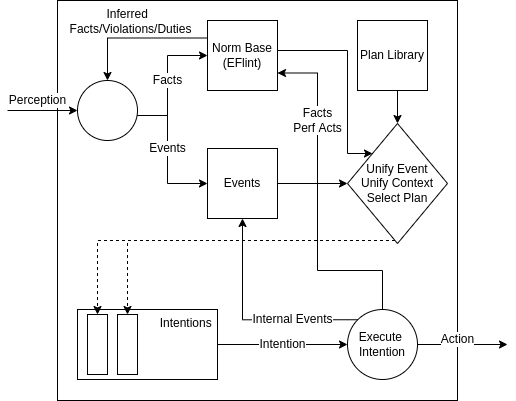
\includegraphics[width=\textwidth]{ch_eumas/nbdi.png}
  \captionof{figure}{Normative advisor's architecture}
  \label{fig:nbdi}
\end{minipage}
\end{figure}
%

This section describes an architecture for advisors and discusses how the ASC2 BDI framework and the eFLINT normative reasoning framework are used to implement the architecture.
%
%
The eFLINT framework is used to implement the norm base.
%
The advisors as well as the intentional agents that employ them are defined in ASC2.
%
Our implementation benefits from the modularity provided by ASC2, allowing easy replacement of different parts of the agent\footnote{ASC2 uses Dependency Injection, meaning most of the dependencies of an agent (e.g. belief-base, communication layer) are passed to it; also, Inversion of Control, meaning higher-level objects (e.g. agent) define a generic control flow and call into lower-level potentially customized objects (e.g. belief-base) to concretize the execution.} and the Java API provided by eFLINT.
%
%Note that most contemporary BDI frameworks that follow the principles of AgentSpeak(L), such as Jason and ASC2, use internal Prolog-like engines as their belief-base. 
%that is also utilized for inferencing new knowledge from facts. This belief-base alongside the agent's plan library and the internal event handling cycle drives the behaviors of the agent. 

\subsection{Normative advisor architecture and decision-making cycle}
Figure~\ref{fig:nbdi} illustrates an overview of the architecture of a normative advisor.
%While AgentSpeak-like languages have high-level abstractions for implementing intentional agents, they do not necessarily provide the proper abstractions for specification of norms, where this level of abstraction is indeed present in norm specification DSLs like eFLINT. On the other hand, while norm specifications generally do not imply concretely the social settings they are applicable in, still they only take meaning in such social settings and having an agent that is aware of the social setting alongside the norms gives much more usability to the norms.
% The architecture in Figure \ref{fig:nbdi}
It is inspired by the BDI architecture of Jason \cite{Bordini2005}.
%
In effect, in this architecture a normative advisor can be seen as a BDI agent in which the (typically Prolog-like) belief-base is replaced the norm reasoner, thus, logical reasoning of the agent is replaced with normative reasoning. Apart from the differences between a logical reasoner (e.g. Prolog) and a norm reasoner (e.g. eFLINT), the main architectural differences of an advisor with a typical BDI agents are: (1) the belief-base (in this case, the norm-base) of the agent can generate more than just belief-update (or fact-update) events, it may now also raise duty events, act (enabled/disabled) events and violation events upon which the agent can react  according to its plan library; (2) from the execution context of a plan alongside fact-update actions (\asc{+fact} and \asc{-fact}), there can now be act-perform actions (\mintinline{text}{#perform(act)}). These differences arise from the the fact that unlike a logical reasoner like Prolog that typically uses backward-chaining to infer facts based on queries, the eFLINT framework also produces information in a forward-chaining manner, thus generating more events for the advisor to process.
%
% With this approach,
Despite these modifications, the core of the AgentScript DSL, and the capabilities of the framework, like goal adoption, communication, and performing arbitrary primitive actions, remain the same as with intentional agents. 
%

Let us analyse a decision-making cycle of the advisor. When the advisor receives an external or internal event, if it is a fact-update, it will be sent to the norm base. 
%
If the event is an achievement or test event, it will be sent to the event queue. 
%
Events are taken from the event queue by an event-selection function, at which moment the head of the event is matched with the plan library to find all the relevant plans. 
%
The context conditions of relevant plans are checked against the normative state of the norm base in order to select only applicable plans. 
%
Then, a plan selection function selects one applicable plan and turns the plan into an intention, and, 
%
consequently, an intention selection function chooses intentions for execution. 
%
If the body of the plan includes any fact-update actions (\asc{+fact} and \asc{-fact}) or act performance  (\mintinline{text}{#perform(act)}), then these are sent to the norm base. 
%
Whenever there is any update committed to the norm base, there could be multiple new events or new facts derived by the normative reasoner that are sent back to the advisor as internal events.

%
These new capabilities are also the result of replacing the Prolog reasoning engine with the eFLINT reasoner.
%
Any Boolean expressions in the DSL can now refer to pre-defined predicates corresponding to eFLINT keywords for querying the norm base: \mintinline{text}{holds/1} is used to check if a fact (or act, duty, etc.) holds, \mintinline{text}{enabled/1} whether the preconditions of an act hold, and \mintinline{text}{violated/1} checks if a duty was violated. 
%
A comprehensive list of possible interactions with the eFLINT norm reasoner is given in the next subsection.
%


\subsection{eFLINT norm base implementation}
%
The eFLINT language is implemented in the form of a reference interpreter in Haskell\footnote{Publicly available online \url{https://gitlab.com/eflint/haskell-implementation}.}.
%
As discussed in~\cite{VanBinsbergen2020EFLINT:Specifications}, the interpreter can run in a `server mode' in which it listens to requests on a certain port and produces responses according to some API.
%
A layer has been developed on top of the server to maintain multiple server instances as is need for supporting multiple advisors with a norm base each.
%
An eFLINT server instance can receive the following \textbf{requests}:
%
\begin{itemize}
\item \textit{Fact creation/termination/obfuscation}. A created fact (instances of fact-types, act-types, duty-types and event-types are referred to as facts) is set to `true' in the knowledge base, a terminated fact to `false' and any existing truth-assignment is removed when a fact is obfuscated.
\item \textit{Triggering an action or event}. Instances of act-types and event-types can be \emph{triggered}, resulting in the effects of the action or event manifesting on the knowledge base (\mintinline{text}{#perform} in Listing~\ref{listing:advisor}). These effects can be to create/terminate/obfuscate certain facts, as listed in the corresponding (post-condition) clauses of the type declaration of the triggered action/event. Note that, because of the synchronization mechanism, multiple actions/events can be triggered at once.
\item \textit{A query in the form of a Boolean expression.} The expression is evaluated in the context of the current knowledge base and can be used to establish whether a certain fact holds true in the current knowledge base, whether an action is enabled (\mintinline{text}{holds} in Listing~\ref{listing:advisor}) or whether a duty is violated, etc.
\item\textit{The submission of a new type declaration} or \textit{the extension of an existing type}. Both have the effect of modifying the norms in the sense that the underlying transition system is modified. %by adding new fact-types, duty-types, act-types and event-types, new derivation rules, new rules to determine the consequences and enabledness of an action, new violation conditions for duties, etc. 
\end{itemize}
Every request can be associated with additional context information in the form of truth-assignment to facts that override any conflicting assignments in the current knowledge base (e.g. the current UNIX time). This mechanism can also be used to provide truth-assigments for `open types' (see below). An eFLINT instance generally operates \textit{synchronously}, i.e. will only send out information in \textbf{responses} to requests\footnote{If necessary, a clock event can be triggered periodically, possibly resulting in synchronous updates.}, updating the sender upon the following:
%
\begin{itemize}
\item Any created, terminated, and/or obfuscated facts. % are reported. 
Note that this includes changes to facts that are (or were previously) derived from other facts and in this sense were indirectly modified by the incoming request
\item Any changes to normative positions regarding duties, i.e. whether a duty is no longer held by an actor or whether a duty is now held by an actor (e.g. \mintinline{text}{-duty} and \mintinline{text}{+duty} in Listing~\ref{listing:advisor}). Violated duties are also reported as such.
\item Any changes to normative positions regarding powers, % and t actions,%\footnote{A power is considered an action with consequences relating to normative positions}
i.e. which actions became (or are no longer) enabled. If the incoming request was triggering one or more actions that were not enabled, the effects of the actions still manifest, but the violations are reported. 
\item In response to a query, the reasoner responds with the result of the query (state is unchanged).
\item If the incoming request requires the evaluation of a fact for which no truth-assignment is given and which is an instance of an `open type'---a type for which the closed world assumption does not hold---then an exception is raised and reported to the sender of the request. Evaluation is interrupted and the state remains unchanged.\footnote{The exception can be used by the parent of the advisor to acquire the missing information, e.g. from another agent in the MAS.}
\end{itemize}
%
All changes to facts' truth-assignment, normative positions and violations register as internal events in the normative advisor (as shown by Listing~\ref{listing:advisor}), which will process and possibly report them according to its script.
%
%The parent of the advisor has to decide whether the actors involved---e.g. in the case of (violations of) duty-claim and power-liability relations---are informed.
%
% The implementation of advisors and the interactions with their parents are discussed next.

\subsection{Spawning and interacting with advisors}
%
\label{sec:scenario}
\begin{listing}[t]
\begin{minted}[fontsize=\small,linenos]{prolog}
+?permitted(A) : enabled(A) => #respond(true).
+?permitted(A) => #respond(false).

+!perform(A) : enabled(A) => #perform(A).
+!perform(A) => #tell(Parent, failed(A)).

+duty(D) => #tell(Parent, D).
-duty(D) => #untell(Parent, D).
\end{minted}
\caption{AgentScript specification of norm advisor.}
\label{asc:advisor}
\label{listing:advisor}
\vspace{-5pt}\end{listing}
%
% Scripts of normative advisors are written in the ASC2 DSL to enable communication between advisors and the parents that spawn them.
%
Scripts of normative advisors (written in ASC2 DSL) run on top of the advisor architecture and give the programmer access to the norm reasoner, both providing its input in the form of queries and updates and responding to the normative events the reasoner generates. In such sense, advisors functionally act as ``bridges'' or chain of transmission between institutional and social realms. 
%
Listing~\ref{listing:advisor} shows a basic script for an advisor in our running example. % that runs on top of the advisor architecture.
%
The advisor has four test-goal plans related to acts and two related to duties.
%
The query \asc{+?permitted/1} receives an act and responds with \mintinline{text}{true} if the given act is ``permitted'' according to the underlying norm reasoner---in the case of eFLINT ``enabled''---and \mintinline{text}{false} otherwise.
%
The agent has similar plans to submit (or not) the performance of acts (\asc{+!perform/1}) to the norm reasoner. 
%
The last two plans are triggered when the internal norm reasoner creates (\asc{+duty/1}) or terminates (\asc{-duty/1}) a duty.
%
The advisor informs their parent of these changes.
%
The fragment demonstrates that observations about created and terminated duties are communicated to the intentional actor (\asc{Parent}) and that an action \textbf{A} can only be performed when it is enabled according to the norm reasoner (or fails otherwise); however this script does not demonstrate all the features possibly delivered by the architecture such as internal events for violations, enabled/disabled acts, and asserted/retracted facts.
%

To demonstrate spawning and interacting with a normative advisor, consider again Listing~\ref{asc:buyer} in which a script for a buyer agent is given.
%
Together, Listings~\ref{asc:buyer}, ~\ref{listing:eflint}, and ~\ref{listing:advisor} show the DSL code for buyer agent in the market-place as presented on the right side of the Figure~\ref{fig:non-gov}.
%
The buyer agent spawns a normative advisor, which in turn spawns an eFLINT server (norm reasoner). 
%
The buyer has its own beliefs and desires: there is a specific item that it needs (\asc{needed_item/1}), it has a belief about the fair price (valuation) for that item (\asc{fair_price/2}) and it has a belief about how much money it possesses (\asc{have_money/1}).
%
When this agent receives a \asc{+offer/2} message about an item and its price, first it interprets it as an \asc{offer} act and sends it to its advisor. Next, it adopts a goal of \asc{consider_buying} that item for the price. This goal has one plan associated to it, which checks if the agent actually needs that item, if the price is considered a fair price and finally if the agent has enough money to buy that item. If this is all true, it sends a \asc{accept/2} message to the agent that made the initial offer. Unlike before, this alone does not constitute performing the normative \asc{accept} act. Instead, it waits until it receives a \asc{+acknowledge/1} message from the seller before communicating acceptance to the advisor. This extra-institutional step for the buyer to qualify the act of \asc{accept}, is an example of context-based qualifications in intentional agents.

\begin{figure}[!tb]
%   \centering
%   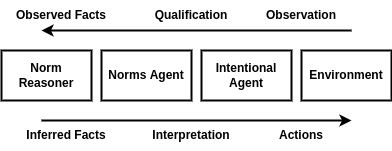
\includegraphics[width=.9\linewidth]{nMAS-drawio.png}
%   \captionof{figure}{Information }
%   \label{fig:}
  \centering
  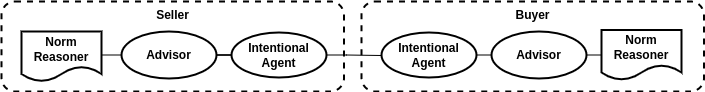
\includegraphics[width=.8\textwidth]{ch_eumas/ad-hoc.drawio.png}
  \captionof{figure}{Market-place model}
  \label{fig:non-gov}
\end{figure}

When the \asc{accept} act is submitted to the norm reasoner, the two previously mentioned duties of \asc{duty_to_pay} and \asc{duty_to_deliver} are generated and sent by the advisor to the intentional part of the Buyer. For the \asc{duty_to_deliver} the agent is the \textit{claimant} (it holds the expectation of performance); it could be that the agent asks the seller agent at this point to deliver the item, but instead, with the implicit assumption that the Seller agent is also compliant to the same set of norms, this agent simply adds this expectation to its belief-base and only when it has an observation of \asc{delivery/2}, it will remove this expectation and send the \asc{deliver} act to the advisor. 

For the \asc{duty_to_pay} the agent is the duty-holder (it has the obligation to perform) and reacts to this duty by adopting the goal \asc{pay/2} (meaning it has the desire to be compliant). There are two plans for this goal, the first one is straightforward and is applicable if the agent has the required amount of money which then it will simply pay the Seller and submits this act to the advisor. However, the second plan (not implemented) is applicable if the agent does not have enough money, which means it needs to find alternative paths to relieve this duty, e.g. by returning the item, borrowing from another agent or even asking another agent to pay the seller instead. Specifying these alternatives requires extensions to either the agents, to the norms, or to both. Rather than working out one or more of these alternatives, we consider different interesting opportunities of extending this straightforward example and reflect on the design of advisors in the next section.  

\section{Discussion}
\label{sec:discussion}

% This p a much desired of concerns that % in a comprehensive way without limiting the concepts of autonomy like their own desires and preferences. The two simple examples showed different ways that such agents can be used to coordinate a MAS. While the examples are rudimentary, they include some important concepts that will be used as the basis of discussion over the approach.


 


%is close to and the normative BDI agents in \cite{Tufis2017} are all examples of works that extend the BDI architecture in ways that enable the agent to take norms (more specifically permissions, obligations and prohibitions) and desires into consideration and possibly resolve conflicts at different levels of agent's logical reasoning varying from norm recognition and norm adoption to decision-making time.

This paper presents an approach to embed (constitutive and regulative) norms into a MAS in a modular and versatile manner, enabling autonomous agents to reason with norms. 
%
In this section we discuss this approach, its connection to certain requirements for a normative MAS, while reflecting on the illustrated example.

Inline with MAS, and distributed computing in general, we consider \textbf{consistency as a consequence} of how a system is set up rather than it being ensured by the framework through which the system is built.
%
This allows for a kind of partial consistency that enables freedom for local deviations that are not harmful to the overall system behavior.
%
In our approach, norm adoption and qualification is done by each individual agent, such that their view on the normative state of the world is dependent on both their script and their (bounded) perception.
%
Particularly desirable for social simulations, we can define agents that adopt and follow the same norms but have different conclusions on the normative state of affairs because they have had different observations.
%
Alternatively, agents do not have to follow the same norms but might still be able to behave in a coordinated fashion.
%
An example of the latter in our sales example is a buyer that believes, on top of the existing norms of our example, that deliveries should be done before payments.
%
The buyer can behave according to their own norms without violating the norms adopted by sellers, even though the norms are different.
%

As presented in the previous sections, our running example shows how \textbf{coordination} between agents is achieved by adopting norms and deciding whether to comply with norms. 
%
The example relies on the agents wanting to comply, and therefore exhibiting coordinated behavior.
%
In more adversarial environments, additional \textit{enforcer} agents can be added to provide (positive and negative) incentives to comply.
%
For example, our marketplace can be extended with an agent that acts like a market authority.
%
% With some capabilities to monitor communication between sellers and buyers and to control to some extent, for example, market participation, such an authority can impose the norms they have adopted on the participants of the marketplace. 
%
By responding to violations raised by their advisor(s), the market authority can apply \textbf{ex-post enforcement} of norms on the market's participants.
%
For example, a buyer refusing to pay can receive a warning or, in the case of continued non-compliance, be banned from the market altogether.
%
This discussion further demonstrates the versatility of our approach: it does not impose \textit{a priori} centralized/decentralized governance or ex-ante/ex-post enforcement. 
%
Instead, our approach gives the system designer the flexibility to choose, design and test what their system requires.


Referring to the requirements in Section \ref{sec:framework}, the notion of \textbf{adopting} was illustrated in the simplest form with the buyer agent in Listing~\ref{asc:buyer} with the \mintinline{text}{#spawn_advisor/3} to adopt a norm as an initial goal. The agents also have the \mintinline{text}{#despawn/1} action to and \textbf{drop} an advisor. 
%(\mintinline{text}{#perform(act)}).
However, by adding extra mechanisms in the agent's script, more complex archetypes can be modelled, e.g. the agent may be programmed to keep a score for a certain norm's (and advisor's) utility to decide if it is an effective norm to keep adopted. 

%
The notion of \textbf{qualification}---necessary to fill the gap between computational forms of law and software~\cite{Boella2014APractice}---
%is a topic of particular importance. Such qualifications can be very complicated, and subject to dispute, particularly in situations that concepts in social and institutional reality do not have a one-to-one matching, thus,
%
%programmability of these qualifications improves the transparency of the system. In our approach, qualification 
can performed at various stages, thanks to the %owing to the 
multitude of programmable layers in our approach.
%but that received so far little attention.
%
An example of qualification in the sale transaction is how a seller agent perceives a \textit{pay} act from a buyer agent.
%
While represented as an act in the norms, in the social reality many different actions can be perceived as a payment, e.g. both direct cash payment or indirect 3rd-party transaction (bank transaction) can be qualified by sellers (and authorities) as the act of paying. While direct cash payment is simpler to qualify for the agent, a bank transfer can be more complicated.
%
This qualification rule could have been encoded in the script of an agent.
%
For example, a bank agent can update a seller that they have received new funds as part of a completed transaction.
%
The seller can then determine whether these funds constitute a payment by a buyer for a particular item, and inform the corresponding advisor.
%
%\textcolor{blue}{needs rewrite and may bring the section about it here:} 
 % on which our approach is based.
%
The same qualification can also be performed purely within norms, specifically as in eFLINT, actions and events are synchronized such that preconditions and effects of %the synchronized 
transitions are effectively `inherited'. % between actions and events.
%
In this way, explicit `counts as' relations between performed actions (transitions) can be specified.
%
% This is % particularly 
% useful to a) connect actions from various normative sources which are simultaneously applicable to a system and b) connect physical behavior to institutional counterparts with possible normative consequences.
%
%For example, through (b) it is possible to connect the concrete actions by (human or software) actors in a system to the rights and obligations laid out in a contract and through (a) to connect actions within the contract to relevant (inter)national law.
%
Listing~\ref{listing:transaction} shows for instance how a transaction event in a banking system is connected with (qualified as) a payment action in our running example. This means the intentional agent only needs to indicate to the advisor that the original event \mintinline{text}{transaction_completed} was triggered which will automatically be inferred as performance of a \mintinline{text}{pay} act.

\begin{listing}[t]
\centering
\begin{tcolorbox}[left=2pt,right=2pt,top=2pt,bottom=2pt,arc=0pt,
                  boxrule=0pt,toprule=1pt,
                  colback=white]
\begin{minted}[fontsize=\small,linenos]{haskell}
Fact account
Placeholder sender    For account
Placeholder receiver  For account
Event transaction-completed 
  Related to sender, receiver, price 
  Syncs with pay(sender, receiver, price) 
    When buyer(sender) && seller(receiver) 
\end{minted}
\end{tcolorbox}
\caption{eFLINT fragment connecting a bank transaction to the \texttt{pay} action.}
\label{listing:transaction}
\vspace{-5pt}\end{listing}

%
% Alternatively, 
%
%In general, our approach enables agents to use all of their capabilities (beliefs, rules, perceptions, planning) to generate messages to advisors for updates to norm instances (\textbf{qualification of social context} in Section~\ref{sec:framework}) and to react to normative events about which they are informed by their advisor(s) (\textbf{qualification of normative concepts} in Section~\ref{sec:framework}).
%

The notions of \textbf{query}, \textbf{update}, \textbf{revert} and \textbf{reset} are already afforded by the norm reasoner where query and update are typically provided by most norm frameworks. However, eFLINT can be used to reason about the compliance of historical, hypothetical, and -- most relevant here -- dynamically developing scenarios:
%
%The type declarations of a specification introduce types of facts, acts, duties and events, which together define a transition system in which states -- knowledge bases of facts -- transition according to the effects of the specified actions and events.
%
%The transitions may output violations if an action triggered a transition with unfulfilled preconditions (e.g. only sellers can make offers) or if any duties are violated in the resulting state. 
%
it 
%has 
relies upon a declarative component that lays out the norms in the form of a labelled transition system and an imperative component that describes traces in this system. This means that similar to belief queries and revision, the agent is able to query and revise (assert/retract) institutional facts. But, unlike physical state, institutional state is revertible as for example, an agent may notice that its observation about performance of an act was not correct or even it wants to infer hypothetical effects of performance of an act before reverting them.


Another important legal/normative requirement is \textbf{adaptability} to new (interpretations of) norms.
%
In our approach, such adaptation can be achieved in at multiple ways.
%
Firstly, apart from spawning new (and despawning old) advisors to start using the new interpretation or encoding of a set of norms, ASC2 agents are able to modify their script at run-time to change the interactions between institutional and social reality, this is true for both intentional agents and advisors. An agent can keep an advisor and its institutional state but instruct the advisor to change how certain events should be handled by modifying its plans. This type of modifications are also present in other BDI frameworks such as Jason.
%
Secondly, an existing advisor can be instructed to update the norm source of an instance it has spawned by adding new type declarations or extending existing types. For example, a violation condition can be dynamically added to the payment duty by submitting the fragment \mintinline[fontsize=\small]{haskell}{Extend Duty duty_to_pay Violated when <EXPR>} for some Boolean expression, like a parameterized timeout event. These types of modifications are particularly interesting as a future work to explore a principled approach for studying changes in the norms such as issues about consistency between variations of norms and impact of norm changes in social simulations.
%
% Both methods raise questions about consistency and migration; that is, does the new norm instance provide the same interface in terms of action, events and duties to interact with, and is the existing institutional perspective (the facts in the norm base) still consistent with the new norms?
%
% A principled approach to handle such adaptations needs to be explored in future work.


However, this does not represent the whole adaptation problem as modification of rules can be much more complex. From the prospective of jurisprudence, laws can be separated into primary and secondary rules~\cite{hart2012concept}; primary rules are about how individuals should act (or not act) and duties that should be fulfilled. Secondary rules are about how primary rules should be created and modified. Typically, normative frameworks (including eFLINT) mainly focus on primary rules while rarely taking secondary rules into account. This means that rather than claiming to solve the whole adaptation/modification problem, we provide a potential starting point to tackle this challenge and believe the fundamental architectural design is adequate to implement other more complex approaches to norm adaptation.



The notions of \textbf{receive and process}/\textbf{ignore} and \textbf{follow}/\textbf{violate} for normative conclusions connect directly to the concept of autonomy in the agent. All of these are are already afforded by ASC2 on the language level (or AgentSpeak(L) in a broader sense) as receive and process/ignore, and, follow/violate are simply a matter of implementing the plans in the agent's script that define the reactions to such conclusions. Then, as the intentional agents' language and execution cycle are not modified in this architecture, intuitively, autonomy of the agents is also not demoted by integration of norms, particularly in comparison with any BDI agent that does not integrate norms. However, as a future work, these concepts-- specially follow/violate-- should be encoded in a more expressive and transparent manner. This can be done, for example, by utilizing declarative constructs such as preferences on the language level (see \cite{Mohajeriparizi2022Preference}) to have an explicit, yet programmable way of ordering between intentional (e.g. desires, goals) and normative (e.g. obligations) dimensions of the agent.

%Qualification refers to how an (or a series of) observation or action in the social context relates to normative concepts and vice-versa. 
%An example of this in the sale transaction
%, while the encoded specifications are already an interpretation of the norms in a sale transaction, still 
%is how a buyer agent perceives an \textit{offer} act from a seller agent, while this is an explicit act in the norms, in the real world many different actions can be perceived as an offer, e.g. simply placing an item in a (real or web) shop can be qualified by buyers (and authorities) as the act of offering. In a real system these qualifications can be very complicated, especially in situations that concepts in social and institutional reality do not have one-to-one matching, thus, having the ability to program these explicitly in a high-level language improves the transparency of the system.


%

% As another example, consider a `reseller' agent that buys items and sells them to others with a possible profit. 
% %
% A simplistic reseller strategy will only sell the items in the agent's inventory and buy items only with sufficient funds.
%
%A more realistic strategy takes advantage of the duties defined in the norms by buying items with the money it expects from future payments and selling items it expects from future deliveries.
%
%Being able to design such scenarios can be an important step towards using MAS to not just create compliant agents/systems, but to perform \textbf{norm-based simulations} to analyze the effects of norms on the agents involved in a system.
%
% For example, more or less stringent deadlines for deliveries and payments may influence the behavior of resellers.
%

% To be used in the development of real systems, our implementation should demonstrate \textbf{scalability} with respect to the amount of agents involved, the sizes of their scripts and the sets of norms being adopted.
% %
% Indeed, the ASC2 framework has been implemented to support large amounts of agents running in parallel.
% %
% The weakest link in terms of scalability in our implementation is the eFLINT interpreter used for normative reasoning.
% %
% %At present, only a reference implementation is available.
% %
% This is because the primary requirement of eFLINT current implementation has been correctness with respect to (formal) definitions of syntax and semantics.
%
%In particular, the interpreter applies a very simple closure algorithm to handle derivation rules (Horn-clauses).
%
%Alternative implementations should be able to offer much faster execution of derivation rules for (subsets of) eFLINT.
%
%For this reason, no (empirical) study into the scalability of our overall approach is provided in this paper.

% \paragraph{Technical Notes}
% There are some design choices in this work, especially in the design of advisory agents, that should be noted. Firstly, this approach required the least amount of modifications to the BDI framework. Only the belief-base of the agent was replaced with the norm reasoner and an interface library between the two was developed. Most BDI frameworks are designed with the capability of interfacing with external reasoning engines and therefore naturally support our approach (\ltvb{@Mostafa, examples?}). Furthermore, the modifications to both the intentional and advisory agents remained internal, leaving their language and external interface untouched. This means that these agents have (backwards) compatibility with already defined systems.


% \paragraph{Take weak interpretation and }


\section{Conclusion}
\label{sec:conclusion}
% focusing on the usage of norms in (evaluation of) coordination. The proposed approach  that can be spawned and used by social agents to reason with norms.

This work presented a theoretical framework for embedding norms in a MAS. It is generally acknowledged that agents in a MAS vastly benefit from utilizing norms for more effective/efficient coordination. Here it was further argued that norms, embodied as institutional views of the state of the environment, need normative advisors to facilitate the bridging between institutional and extra-institutional realms. The proposed architecture included using a BDI framework and a norm reasoning framework for creating normative advisors and was shown to address the main requirements of normative (multi-agent) systems as identified by the community. A practical running implementation of this architecture\footnote{publicly available: anonymized} using mostly off-the-shelf tools was presented via a market example to further illustrate the applicability of the approach.

As autonomous agents, norms, and their interactions deal with notions and constructs hard to concretize and on which it may be hard to reach an agreement, they may have different definitions and usages in different scientific communities. Alongside the proposal of the architecture and tools in themselves, this work assumed a high priority for flexibility as a requirement in frameworks utilized in designing normative (multi-agent) systems by proposing multiple programmable components varying from pure context-free and abstract norm specifications to perception/action layer of intentional agents. These components aimed at satisfying the higher level requirements of normative agents and (multi-agent) systems without putting any constraint on the language or logic used in components.



